\chapter{Results}
TODO: This chapter will....
\section{Goals}
We study how the extension of KG affects rule mining, and the role of extension methods in the process. Some central questions here are:
\begin{enumerate}
    \item Does adding new plausible facts lead to new rules being mined? 
    \item How does the PCA confidence of these rules compare to the rules mined from the original KG?
    \item Can the rules mined from the original KG also be mined after the KG is extended?
\end{enumerate}
Regarding extension methods we will look at three parameters:
\begin{itemize}
    \item the \textit{entity selection strategy} for candidate generation
    \item the \textit{KG embedding model architecture} for ranking candidates
    \item the \textit{rank cutoff value} for admitting candidates to the KG
\end{itemize}
and their role in the quantity and PCA confidence of the rules that are mined.
\section{Overview of results}
This section will give a brief overview of the results and focuses on the fact that most of the rules mined derive from KGs extended using TransE.
\subsection{KG extension sizes}
In the KG extension process there are 48 \footnote{4 (KG embedding models) $\times$ 4 (entity selection methods) $\times$ 3 (rank cutoff) = 48 parameter combinations.} different parameter combinations. This means that there are 48 different KG extensions for each original KG. Extension set sizes range from approximately 800 to 33500 triples, where the RandomBaseline model admitted the most candidates. This makes sense, as the models assign a random score to facts, so that many more receive a high rank. The \textit{trained} models give most candidates a low score because most triples usually are bad candidates. Note that the extension sizes were about the same for both datasets, while WN18RR and the family KG respectively have 88 227 and 258 235 facts, therefore the extensions for WN18RR are relatively larger than for the family KG.

\subsection{Rule set sizes and mean PCA confidence}
\label{TransE_sucks} 
Upon examining the number of rules mined per KG extension one immediately sees some startling results. Most rule sets don't differ drastically in size, apart from those where TransE was used, where these rule sets are \textit{exceptionally} larger. See \cref{all_sets} in the appendix to observe the difference. When looking at the mean PCA confidence of the rules sets one also notes that the score for the TransE sets are mostly around 0.1, while the remaining rule sets have a score on average around 0.5.

\begin{figure}[h]
\centering
\begin{subfigure}{.5\textwidth}
  \centering
  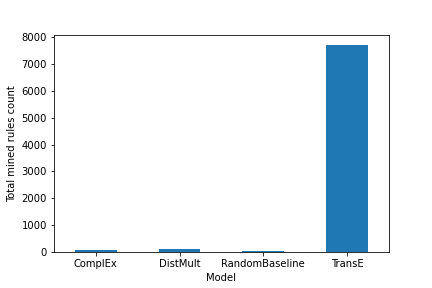
\includegraphics[width=1\linewidth]{figures/results/Total_mined_rules-model-wn18rr.png}
  \caption{WN18RR}
  \label{fig:sub1}
\end{subfigure}%
\begin{subfigure}{.5\textwidth}
  \centering
  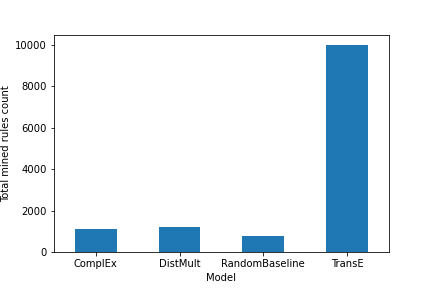
\includegraphics[width=1\linewidth]{figures/results/Total_mined_rules-model-family.png}
  \caption{Family KG}
  \label{fig:sub2}
\end{subfigure}
\caption{Distribution of number of mined rules over different embedding models.}
\label{fig:test}
\end{figure}

As discussed in Section \ref{TransE_peaked_in_2013} TransE is not able to learn certain relation qualities, and upon further inspection of the embedding vectors for relations in TransE the vector values all tend toward zero. It seems that while scoring decently on the performance metrics during model selection, TransE has not properly embedded the relations in the KG. Of the rules mined, \textcolor{red}{97}\% (WN18RR) and \textcolor{red}{76}\% (family KG) originate from KGs extended using TransE. The large number of rules produced marginalize those mined using other embedding models. Due to this and the fact that the trained TransE model has poor relational embeddings, we will include rules mined from KGs extended with TransE only when examining embedding models, but not when looking at entity selection methods or rank cutoff values.

\begin{lstlisting}[mathescape=true, float, caption={Selection of nonsense rules mined from KGs extended with TransE.},captionpos=b, label={TransE_nonsense_rules}]
$spouse(x, y)  \Rightarrow father(x, y)$
$mother(x, y)   \Rightarrow child(x, y)$
$relative(y, x) \Rightarrow sibling(x, y)$
$spouse(a, y) \Rightarrow child(x,y)$
$relative(x, y) \Rightarrow sibling(x, y)$
$relative(x, z) \wedge sibling(z, y) \Rightarrow mother(x, y)$
$child(z, x) \wedge mother(z,y) \Rightarrow spouse(x, y)$
$relative(y, x) \wedge sibling(y, x) \Rightarrow father(x, y)$
$mother(z, y) \wedge mother(x, z) \Rightarrow child(x, y)$
$sibling(y, x) \wedge spouse(x, y) \Rightarrow father(x, y)$
\end{lstlisting}

\section{Effect of parameters}
In this section we will examine the effects of each of the three main parameters in the KG extension process. Note that when looking at rules with a certain parameter the sets of rules will be a concatenation of all cases where that parameter was used. For example, if we look at the rules mined with ComplEx as the KG embedding model, then this group will contain rules mined from 12 different KG extensions because we need to look at all the combinations of entity selection methods and rank cutoff values ($4\times3=12$). This is differentiated from the case where we look at rules mined from a single extended KG, which we will do in \cref{Rule_comparison}.

\begin{figure}
\centering
    \centering
    \includesvg[inkscapelatex=false,width=1\textwidth,keepaspectratio]{figures/results/rule_dist_models_hbar_family.svg}
    \caption{Distribution of rules over KG embedding models on the family KG.}
    \label{rule_dist_models_hbar_family}
\end{figure}

\begin{figure}
\centering
    \centering
    \includesvg[inkscapelatex=false,width=1\textwidth,keepaspectratio]{figures/results/rule_dist_models_hbar_wn18rr.svg}
    \caption{Distribution of rules over KG embedding models on the WN18RR KG.}
    \label{rule_dist_models_hbar_wn18rr}
\end{figure}


\subsection{Effect of KG embedding model}
At the first glance of boxplots \ref{fig:PCA_models_wn18rr_boxplot} and \ref{fig:PCA_models_family_boxplot} it may seem odd that the PCA confidence of rules mined from RandomBaseline extensions is so high. Boxplots are used to represent the spread of data through their quartlies \cite{dutoit2012graphical}. The box itself covers $Q_1-Q_3$, with the horizontal line in the box marking the median. The median PCA confidence for the original rules is indicated by the dashed line across the plots. The boxplots used in this thesis also have \textit{whiskers}, which are the lines extending vertically out of the box. Whiskers give an indication of the variability of the data outside the upper and lower quartiles (respectively $Q_1$ and $Q_3$). Points beyond the whiskers are considered outliers.

\begin{figure}[h]
\centering
\begin{subfigure}{.5\textwidth}
  \centering
  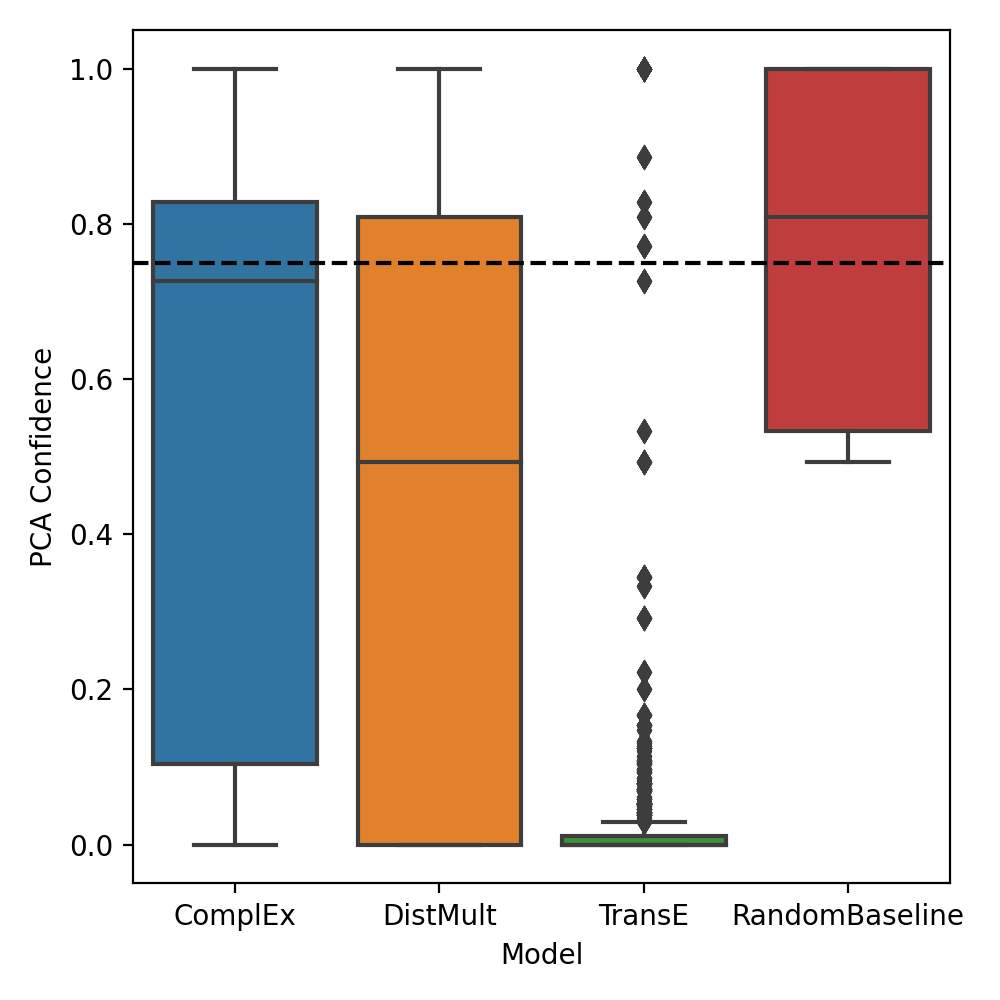
\includegraphics[width=1\linewidth]{figures/results/PCA_models/PCA-models_wn18rr.png}
  \caption{Original KG}
  \label{fig:PCA-models_wn18rr_boxplot_sub}
\end{subfigure}%
\begin{subfigure}{.5\textwidth}
  \centering
  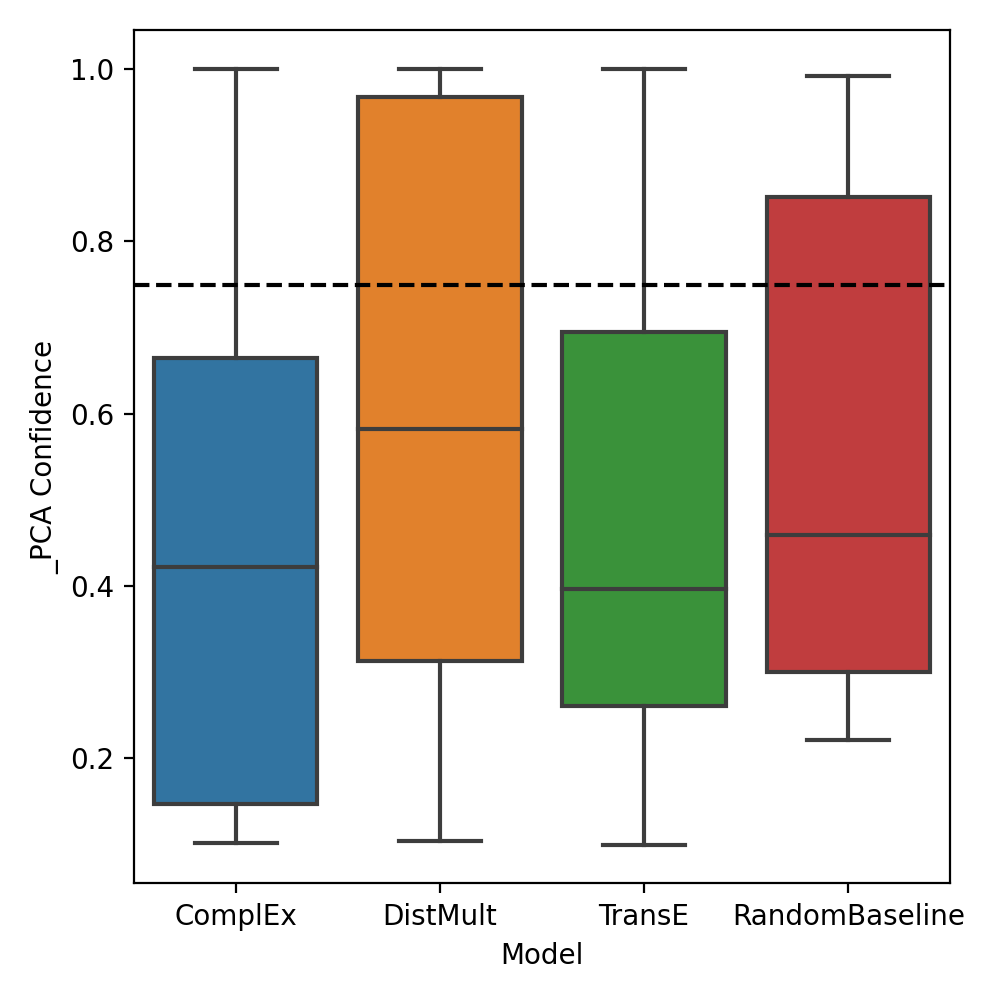
\includegraphics[width=1\linewidth]{figures/results/PCA_models/_PCA-models_wn18rr.png}
  \caption{Extended KG}
  \label{fig:_PCA_models_wn18rr_boxplot_sub}
\end{subfigure}
\caption{Distribution of PCA confidence of mined rules by KG embedding models. PCA confidence scores are calculated on the original WN18RR and the extended WN18RR from which the rules are mined. The dashed line represents the median PCA confidence of the rules mined from the original WN18RR KG.}
\label{fig:PCA_models_wn18rr_boxplot}
\end{figure}

\begin{figure}[h]
\centering
\begin{subfigure}{.5\textwidth}
  \centering
  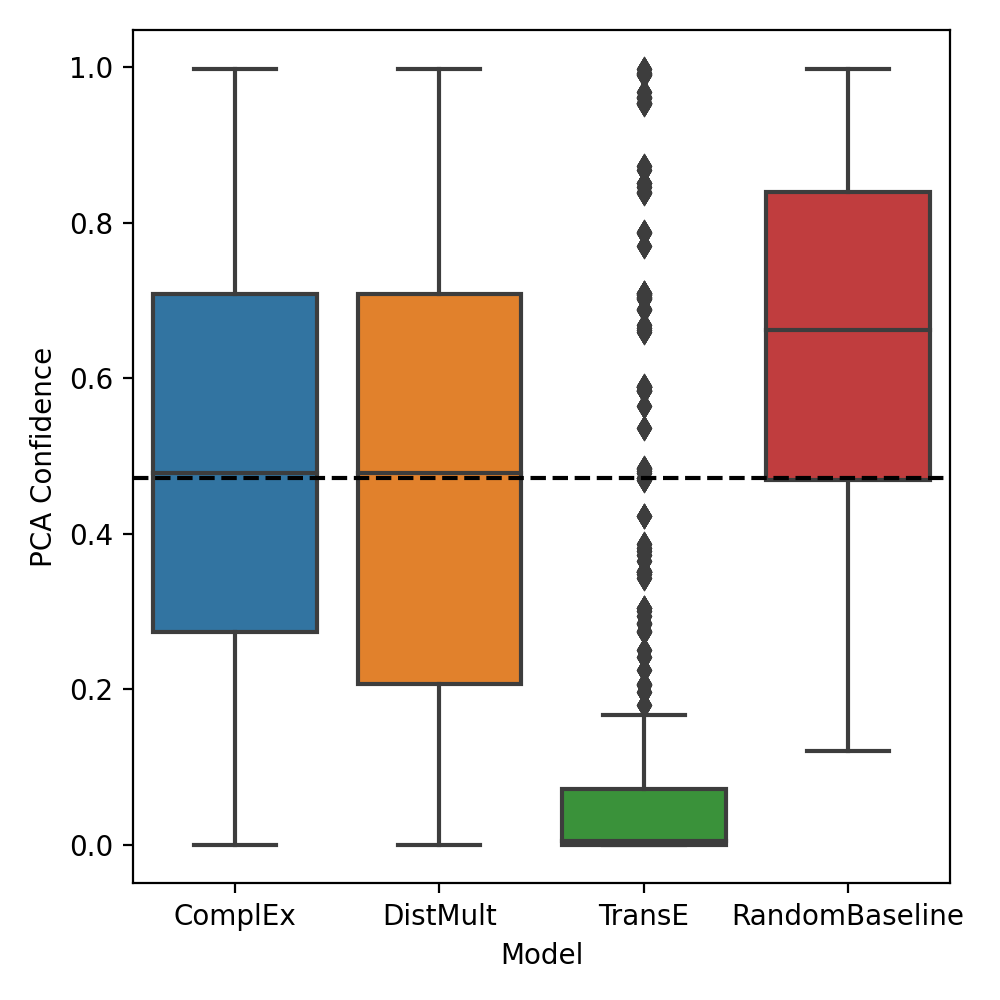
\includegraphics[width=1\linewidth]{figures/results/PCA_models/PCA-models_family.png}
  \caption{Original KG}
  \label{fig:models_family_boxplot_sub}
\end{subfigure}%
\begin{subfigure}{.5\textwidth}
  \centering
  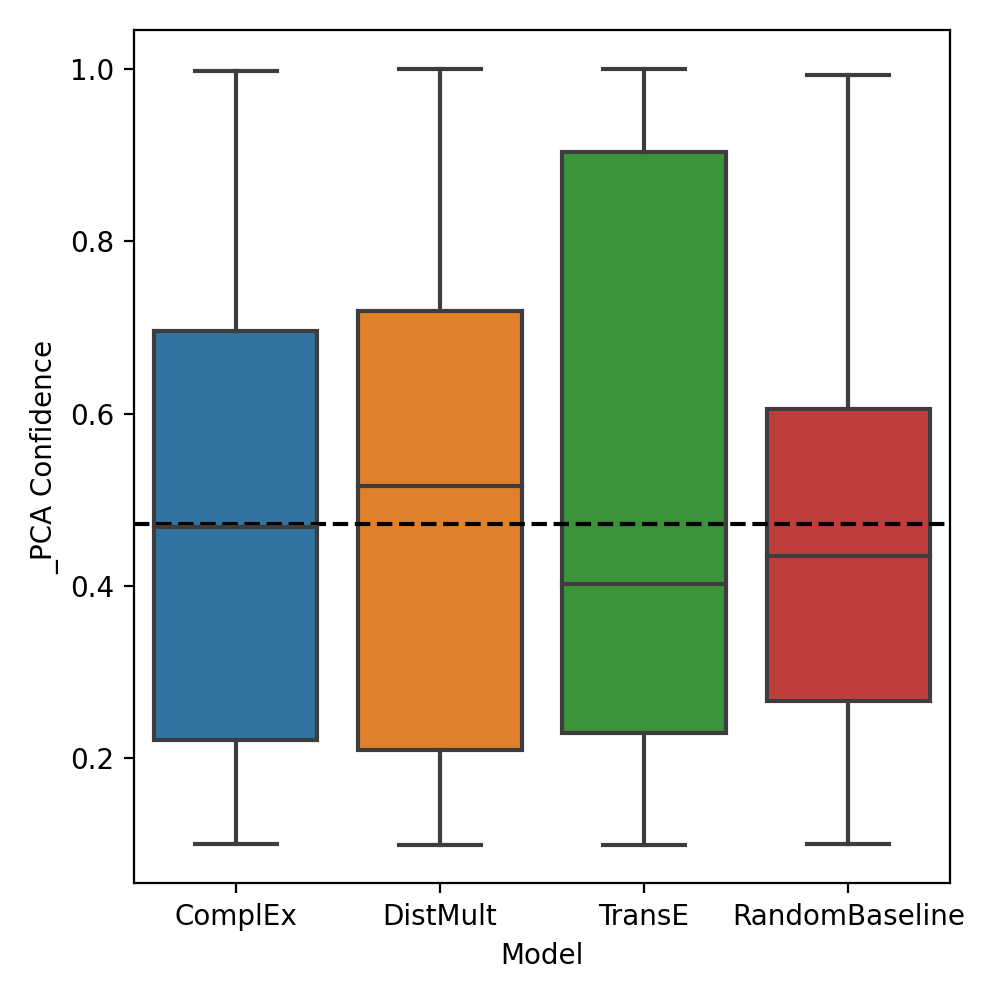
\includegraphics[width=1\linewidth]{figures/results/PCA_models/_PCA-models_family.png}
  \caption{Extended KG}
  \label{fig:_PCA_models_family_boxplot_sub}
\end{subfigure}
\caption{Distribution of PCA confidence of mined rules by KG embedding models. PCA confidence scores are calculated on the original family KG and the extended family KG from which the rules are mined. The dashed line represents the median PCA confidence of the rules mined from the original family KG.}
\label{fig:PCA_models_family_boxplot}
\end{figure}

By looking at figures \ref{rule_dist_models_hbar_family} and \ref{rule_dist_models_hbar_wn18rr} it becomes apparent that there in fact fewer different rules mined from these extensions. In the WN18RR case no new rules were found, and a single original rule was also never mined. The omitted rule,
\[derivationally\_related\_form(x, y)   \Rightarrow derivationally\_related\_form(y, x)\]
has the lowest PCA confidence out of all the original rules. Since there already was little support in the KG for the rule, the addition of noise may have obscured too much evidence for the relation \textcolor{red}{\texttt{derivationally\_related\_form}} being symmetric for the algorithm to consider the rule significant. 
% check RandomBaseline_original_rules.ipynb to see if there is a new rule.

\begin{table}[htp]
\centering
\begin{tabular}{l|cc|cc|cc}
\multicolumn{1}{c}{\multirow{2}{*}{\textbf{Model}}} & \multicolumn{2}{c}{\textbf{Original rules}} & \multicolumn{2}{c}{\textbf{New rules}} & \multicolumn{2}{c}{\textbf{Orig. not found}}         \\
\multicolumn{1}{c}{}                                & Count    & \% of mined    & Count  & \% of mined & Count & \multicolumn{1}{c}\% of original \\ \hline
Baseline                                            & 85             & 100\%                      & 0            & 0\%                     & 9           & 10\%                                           \\
TransE                                              & 94             & 9\%                        & 986          & 91\%                    & 0           & 0\%                                            \\
DistMult                                            & 93             & 51\%                       & 90           & 49\%                    & 1           & 1\%                                            \\
ComplEx                                             & 94             & 69\%                       & 43           & 31\%                    & 0           & 0\%                                           
\end{tabular}
\caption{Distribution of all the rules mined over KG embedding models. KG: family KG.}
\label{Tab:table_rules_models_family}
\end{table}

\begin{table}[htp]
\centering
\begin{tabular}{l|cc|cc|cc}
\multicolumn{1}{c}{\multirow{2}{*}{\textbf{Model}}} & \multicolumn{2}{c}{\textbf{Original rules}} & \multicolumn{2}{c}{\textbf{New rules}} & \multicolumn{2}{c}{\textbf{Orig. not found}}         \\
\multicolumn{1}{c}{}                                & Count    & \% of mined    & Count  & \% of mined & Count & \multicolumn{1}{c}\% of original \\ \hline
Baseline                                            & 9             & 100\%                      & 0            & 0\%                     & 1           & 10\%                                           \\
TransE                                              & 10             & 1\%                        & 659          & 99\%                    & 0           & 0\%                                            \\
DistMult                                            & 10             & 67\%                       & 5           & 33\%                    & 0           & 0\%                                            \\
ComplEx                                             & 10             & 59\%                       & 7           & 41\%                    & 0           & 0\%                                           
\end{tabular}
\caption{Distribution of all the rules mined over KG embedding models. KG: WN18RR.}
\label{Tab:table_rules_models_wn18rr}
\end{table}

The family KG produced similar results, where AMIE3 failed to find 12 original rules in the RandomBaseline-extended KGs. All of these rules were among those with the lowest PCA confidence of the original rules. When the rules with lowest PCA condifence in a set are removed, then the median PCA confidence naturally goes up. This explains how the RandomBaseline rules have a higher median PCA confidence than the original, shown in tables \ref{Tab:table_rules_models_family} and \ref{Tab:table_rules_models_wn18rr}.

As presented in \cref{TransE_sucks}, AMIE3 mines a great deal more rules from KGs extended with TransE. Due to the low mean PCA confidence for these rules (0.038 for WN18RR and 0.089 for the family KG) it is clear that there is little support for the rules in the original KGs. If one however evaluates the TransE rules on the \textit{extended} KGs they were mined from, the PCA confidence increases substantially, as seen in figures \ref{fig:_PCA_models_wn18rr_boxplot_sub} and \ref{fig:_PCA_models_family_boxplot_sub}. So even though most of these rules have little support from the original KGs, it was no mistake that AMIE3 mined so many rules from the TransE-extended KGs.


DistMult and ComplEx are closely related embedding models as they have similar scoring functions (the scoring function of ComplEx corresponds to that of DistMult but with real embeddings), and perform similarly on benchmark datasets \cite{complEx}. As mentioned in \cref{TransE_peaked_in_2013}, DistMult is not able to represent asymmetric relations. Although AMIE3 can only mine Horn rules, thereby a rule defining the asymmetry of a relation cannot be mined, this may still affect the the quality of the embedding and thus the KG extension. From the results it seems that ComplEx is a somewhat stricter model, in the sense that it ranks candidate triples lower against corrupted triples than DistMult does. This is evidenced by the fact that the KG extension sizes are larger for DistMult than for ComplEx; DistMult is admitting more candidates. For example, of the candidates generated with the entity selection method "probabilistic" from the WN18RR KG, DistMult assigned \textcolor{red}{1468} candidates rank 1 while ComplEx only did this for \textcolor{red}{866} candidates. As a result, more rules are mined from DistMult-extended KGs.

The combined set of rules found from ComplEx-extended KGs include all the original rules, both for WN18RR and the family KG.  This is almost also the case for DistMult, but it fails to find the original rule $child(x, y) \Rightarrow mother(y,x)$ in the family KG. This rule has the second lowest PCA confidence of all the original family KG rules.

\iffalse
    \begin{figure*}[h]
        \centering
        \begin{subfigure}[b]{0.49\textwidth}
            \centering
            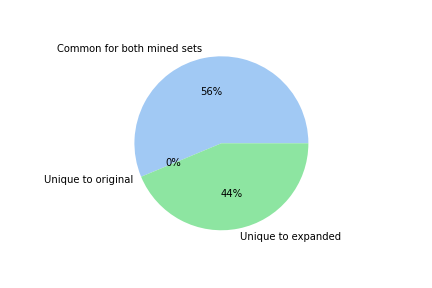
\includegraphics[width=\textwidth]{figures/results/pie_charts-model/complEx_family.png}
            \caption[complEx_pie]%
            {{\small ComplEx}}    
            \label{fig:complex_pie_family}
        \end{subfigure}
        \hfill
        \begin{subfigure}[b]{0.49\textwidth}  
            \centering 
            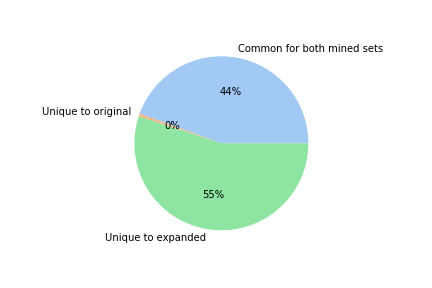
\includegraphics[width=\textwidth]{figures/results/pie_charts-model/distMult_family.png}
            \caption[]%
            {{\small DistMult}}    
            \label{fig:distMult_pie_family}
        \end{subfigure}
        \vskip\baselineskip
        \begin{subfigure}[b]{0.49\textwidth}   
            \centering 
            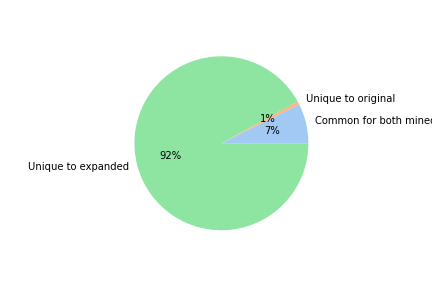
\includegraphics[width=\textwidth]{figures/results/pie_charts-model/transE_family.png}
            \caption[]%
            {{\small TransE}}    
            \label{fig:trasE_pie_family}
        \end{subfigure}
        \hfill
        \begin{subfigure}[b]{0.49\textwidth}   
            \centering 
            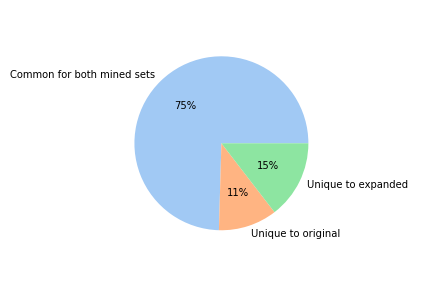
\includegraphics[width=\textwidth]{figures/results/pie_charts-model/randomBaseline_family.png}
            \caption[]%
            {{\small RandomBaseline}}    
            \label{fig:randomBaseline_pie_family}
        \end{subfigure}
        \caption[ The average and standard deviation of critical parameters ]
        {\small Distribution of all the rules mined over KG embedding models. KG: family KG.} 
        \label{fig:model_pies_family}
    \end{figure*}
    
    
    \begin{figure*}[h]
        \centering
        \begin{subfigure}[b]{0.49\textwidth}
            \centering
            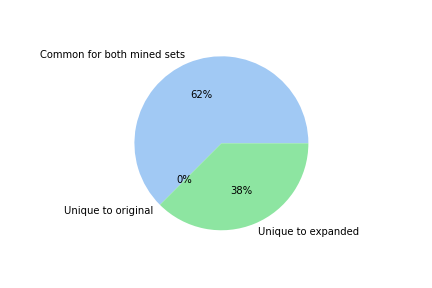
\includegraphics[width=\textwidth]{figures/results/pie_charts-model/complEx_wn18rr.png}
            \caption[complEx_pie]%
            {{\small ComplEx}}    
            \label{fig:complex_pie_wn18rr}
        \end{subfigure}
        \hfill
        \begin{subfigure}[b]{0.49\textwidth}  
            \centering 
            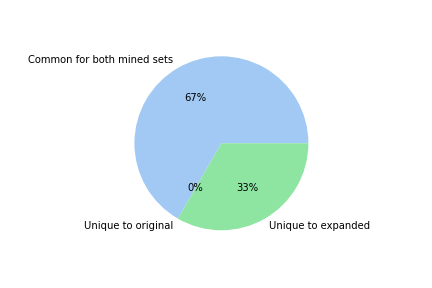
\includegraphics[width=\textwidth]{figures/results/pie_charts-model/distMult_wn18rr.png}
            \caption[]%
            {{\small DistMult}}    
            \label{fig:distMult_pie_wn18rr}
        \end{subfigure}
        \vskip\baselineskip
        \begin{subfigure}[b]{0.49\textwidth}   
            \centering 
            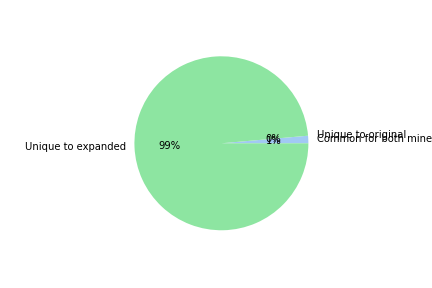
\includegraphics[width=\textwidth]{figures/results/pie_charts-model/transE_wn18rr.png}
            \caption[]%
            {{\small TransE}}    
            \label{fig:trasE_pie_wn18rr}
        \end{subfigure}
        \hfill
        \begin{subfigure}[b]{0.49\textwidth}   
            \centering 
            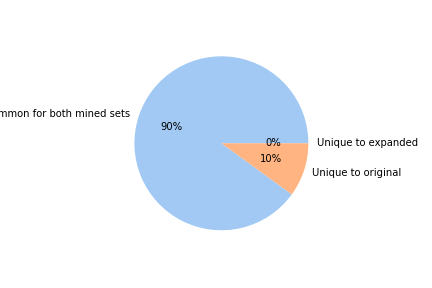
\includegraphics[width=\textwidth]{figures/results/pie_charts-model/randomBaseline_wn18rr.png}
            \caption[]%
            {{\small RandomBaseline}}    
            \label{fig:randomBaseline_pie_wn18rr}
        \end{subfigure}
        \caption[ The average and standard deviation of critical parameters ]
        {\small Distribution of all the rules mined over KG embedding models. KG: WN18RR.} 
        \label{fig:model_pies_wn18rr}
    \end{figure*}

\fi

\newpage
\subsection{Effect of entity selection method}
The \textit{probabilistic}, \textit{random}, and the \textit{least frequent} entity selection strategies perform relatively similarly if we look at the PCA confidence box plots in figures \ref{fig:PCA_entity_wn18rr_boxplot} and \ref{fig:PCA_entity_family_boxplot}. The \textit{most frequent} strategy, however, performs worse, both on the WN18RR and family KG. This is consistent with AmpliGraph's assumption that the most frequent entities are less likely to have missing facts \cite{kge_tutorial}.

In the WN18RR KG all original rules were found, but in the family KG only the \textit{least frequent} strategy resulted in all the original rules being mined. It also resulted in the least new rules being mined, while the \textit{most frequent} strategy led to the most new rules.

Overall it seems like \textit{probabilistic}, \textit{random}, and the \textit{least frequent} entity selection strategies all are appropriate in regard to maintaining PCA confidence. If however the goal is to mine many new rules then \textit{most frequent} apears to be best suited, though at the sacrifice of PCA confidence.

\begin{figure}[h]
\centering
\begin{subfigure}{.5\textwidth}
  \centering
  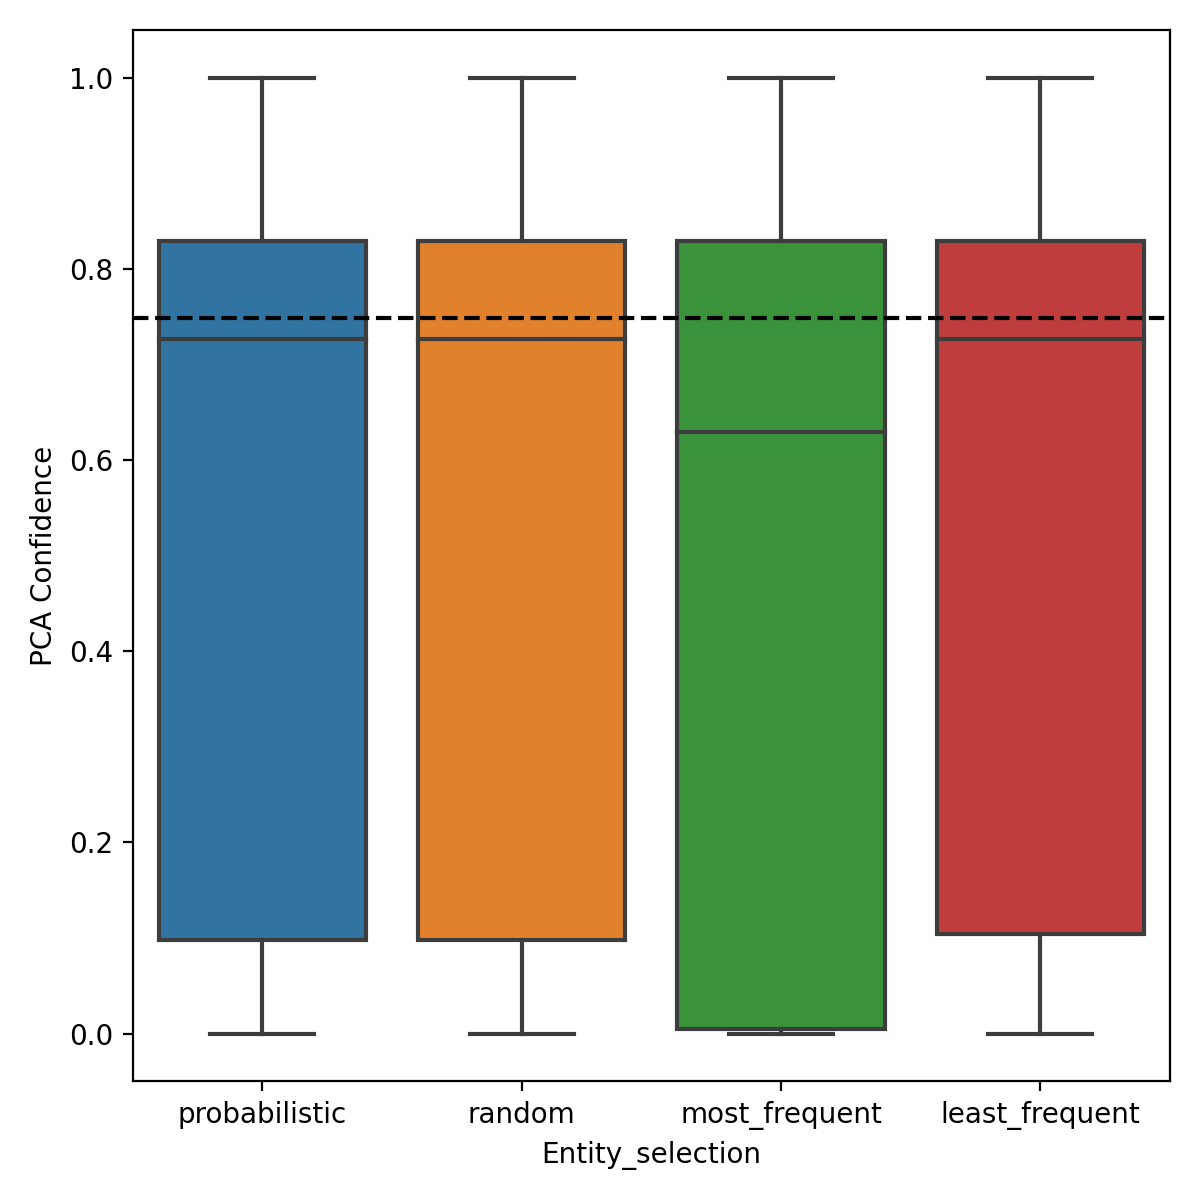
\includegraphics[width=1\linewidth]{figures/results/entity_selection/PCA-entity_wn18rr.png}
  \caption{Original KG}
  \label{fig:PCA-entity_wn18rr_boxplot_sub}
\end{subfigure}%
\begin{subfigure}{.5\textwidth}
  \centering
  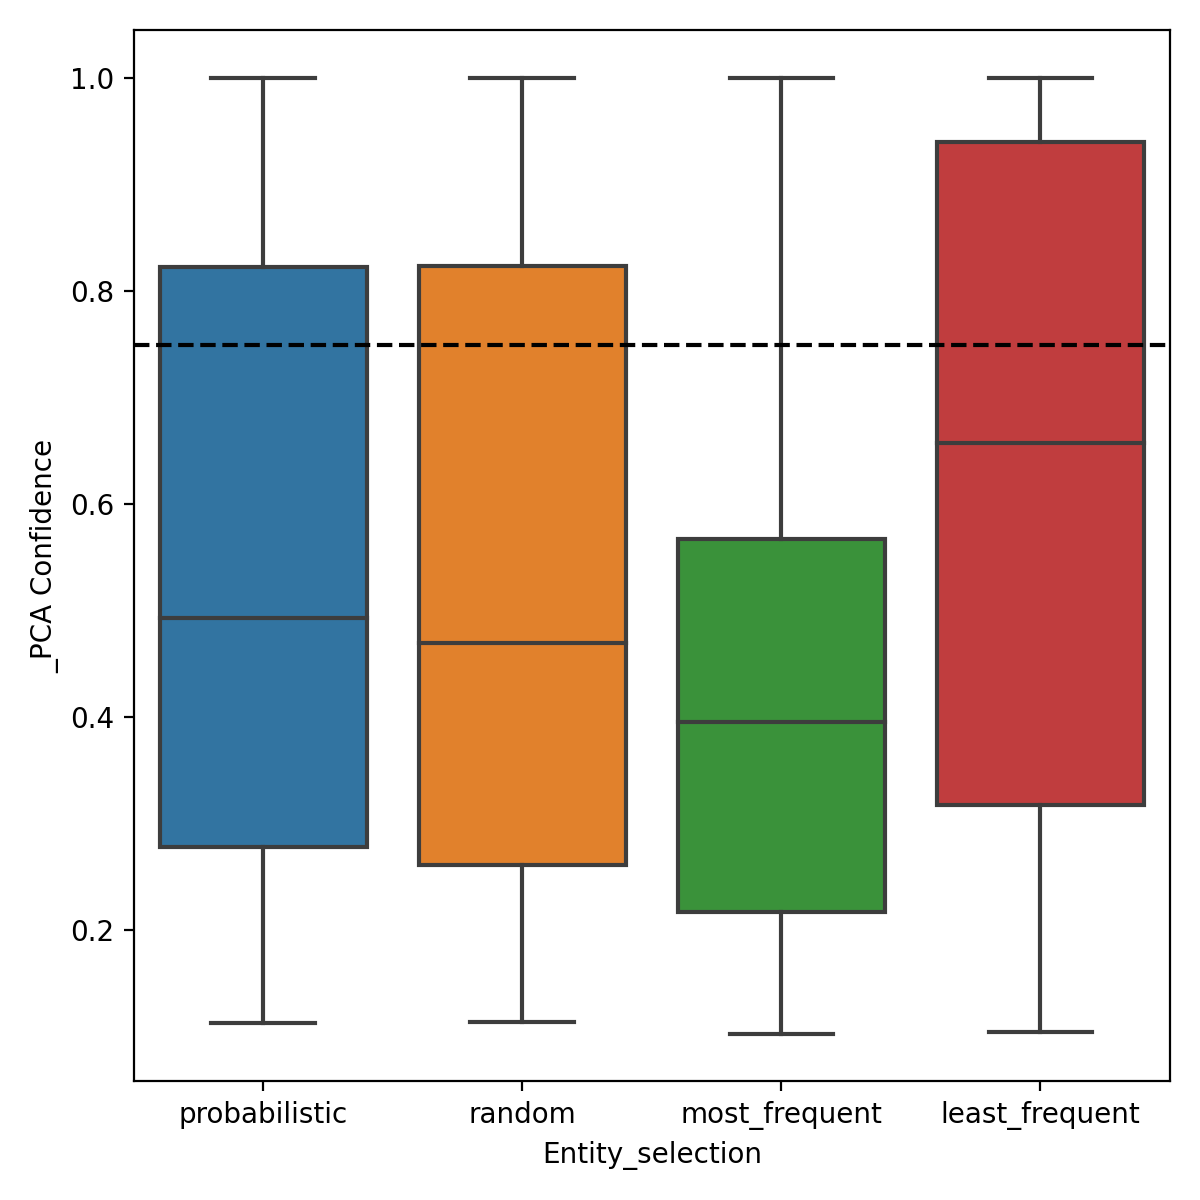
\includegraphics[width=1\linewidth]{figures/results/entity_selection/_PCA-entity_wn18rr.png}
  \caption{Extended KG}
  \label{fig:_PCA_entity_wn18rr_boxplot_sub}
\end{subfigure}
\caption{Distribution of PCA confidence of mined rules by entity selection strategies. PCA confidence scores are calculated on the original WN18RR and the extended WN18RR from which the rules are mined. The dashed line represents the median PCA confidence of the rules mined from the original WN18RR KG.}
\label{fig:PCA_entity_wn18rr_boxplot}
\end{figure}

\begin{figure}[h]
\centering
\begin{subfigure}{.5\textwidth}
  \centering
  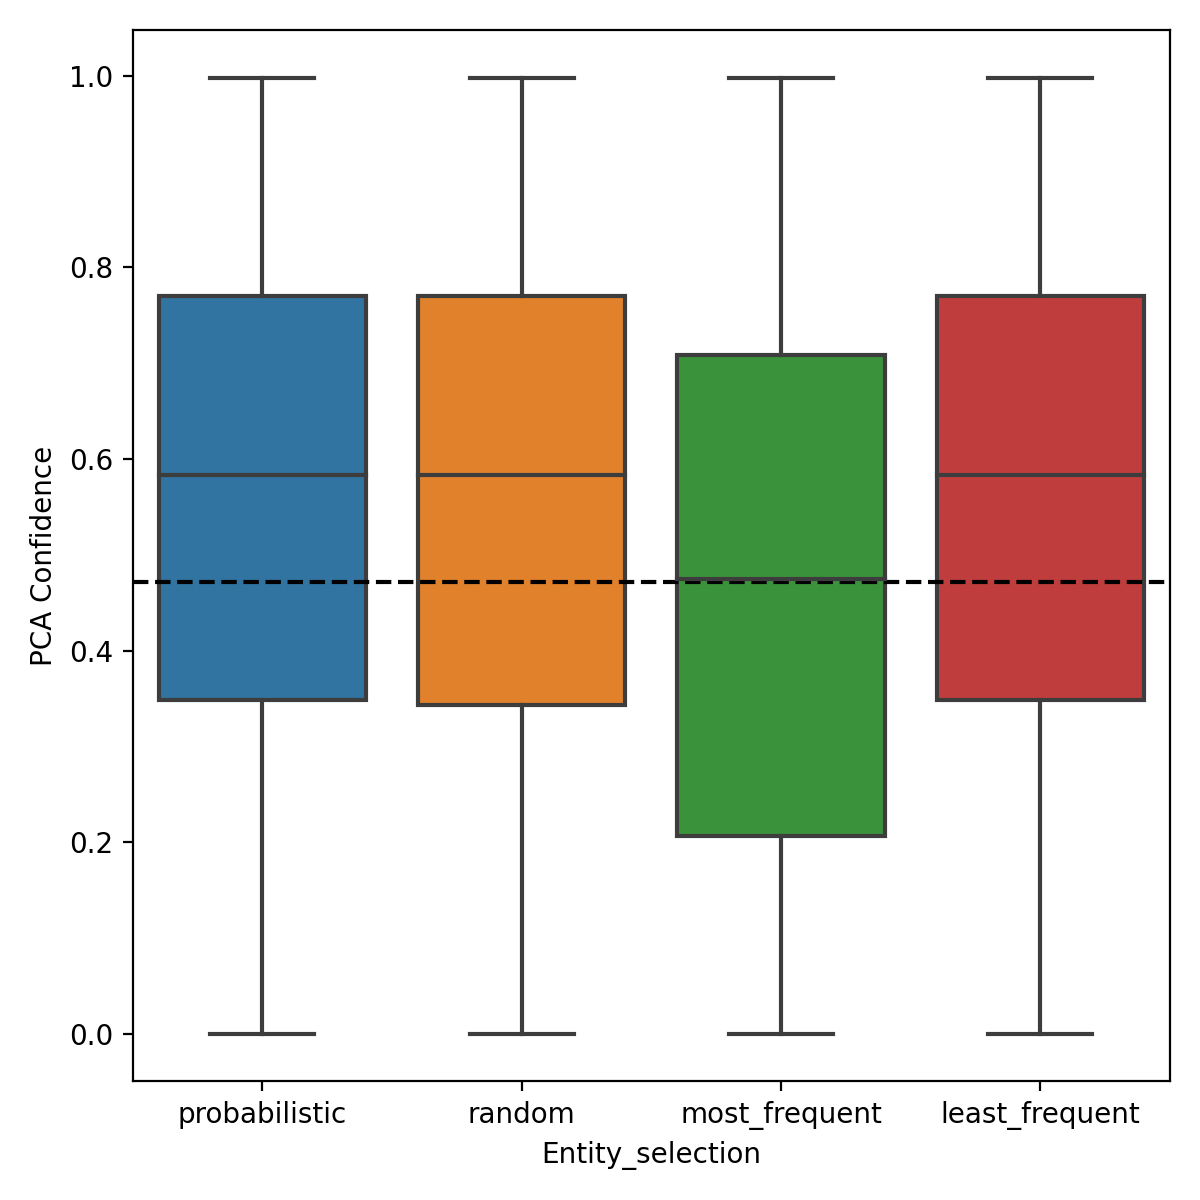
\includegraphics[width=1\linewidth]{figures/results/entity_selection/PCA-entity_family.png}
  \caption{Original KG}
  \label{fig:models_entity_boxplot_sub}
\end{subfigure}%
\begin{subfigure}{.5\textwidth}
  \centering
  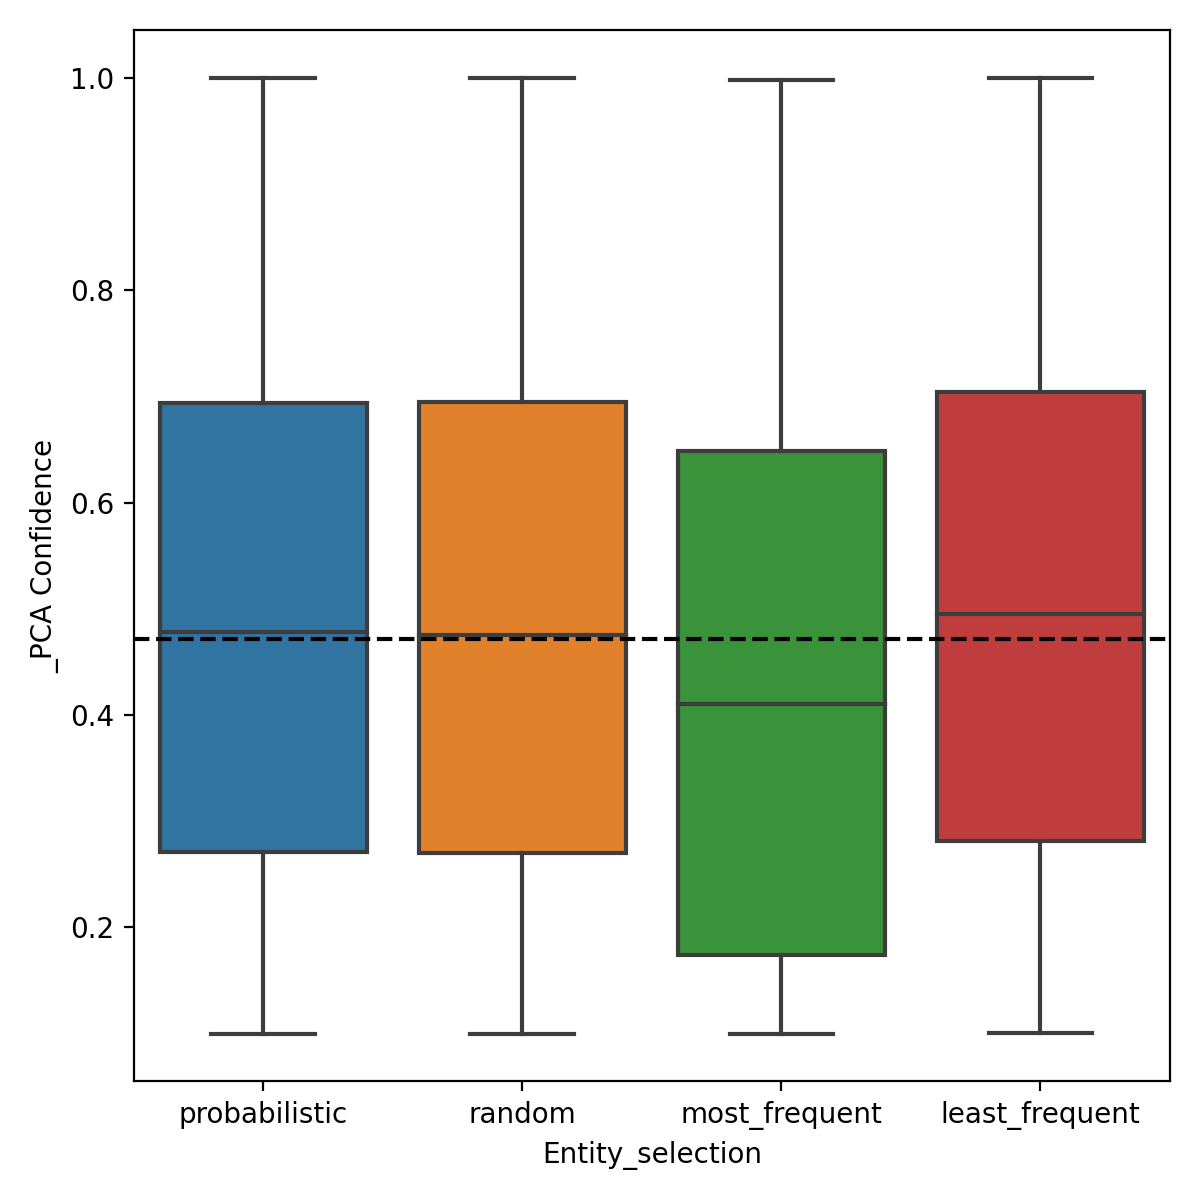
\includegraphics[width=1\linewidth]{figures/results/entity_selection/_PCA-entity_family.png}
  \caption{Extended KG}
  \label{fig:_PCA_entity_family_boxplot_sub}
\end{subfigure}
\caption{Distribution of PCA confidence of mined rules by entity selection strategies. PCA confidence scores are calculated on the original family KG and the extended family KG from which the rules are mined. The dashed line represents the median PCA confidence of the rules mined from the original family KG.}
\label{fig:PCA_entity_family_boxplot}
\end{figure}

\begin{table}[htp]
\centering
\begin{tabular}{l|cc|cc|cc}
\multicolumn{1}{c}{\multirow{2}{*}{\textbf{Strategy}}} & \multicolumn{2}{c}{\textbf{Original rules}} & \multicolumn{2}{c}{\textbf{New rules}} & \multicolumn{2}{c}{\textbf{Orig. not found}}         \\
\multicolumn{1}{c}{}                                & Count    & \% of mined    & Count  & \% of mined & Count & \multicolumn{1}{c}\% of original \\ \hline
Random                                            & 90             & 71\%                      & 36            & 29\%                     & 4           & 4\%                                           \\
Most freq.                                              & 88             & 46\%                        & 105          & 54\%                    & 6           & 6\%                                            \\
Least freq                                            & 94             & 77\%                       & 28           & 33\%                    & 0           & 0\%                                            \\
Probabilistic                                             & 91             & 73\%                       & 33           & 27\%                    & 3           & 3\%                                           
\end{tabular}
\caption{Distribution of all the rules mined over entity selection strategies for the family KG.}
\label{Tab:table_rules_entities_family}
\end{table}

\begin{table}[htp]
\centering
\begin{tabular}{l|cc|cc|cc}
\multicolumn{1}{c}{\multirow{2}{*}{\textbf{Strategy}}} & \multicolumn{2}{c}{\textbf{Original rules}} & \multicolumn{2}{c}{\textbf{New rules}} & \multicolumn{2}{c}{\textbf{Orig. not found}}         \\
\multicolumn{1}{c}{}                                & Count    & \% of mined    & Count  & \% of mined & Count & \multicolumn{1}{c}\% of original \\ \hline
Random                                            & 10             & 53\%                      & 9            & 47\%                     & 0           & 0\%                                           \\
Most freq.                                              & 10             & 42\%                        & 14          & 58\%                    & 0           & 0\%                                            \\
Least freq.                                            & 10             & 48\%                       & 11           & 52\%                    & 0           & 0\%                                            \\
Probabilistic                                             & 10             & 45\%                       & 12           & 55\%                    & 0           & 0\%                                           
\end{tabular}
\caption{Distribution of all the rules mined over entity selection strategies. KG: WN18RR.}
\label{Tab:table_rules_entities_wn18rr}
\end{table}

\iffalse
\begin{figure*}[h]
        \centering
        \begin{subfigure}[b]{0.49\textwidth}
            \centering
            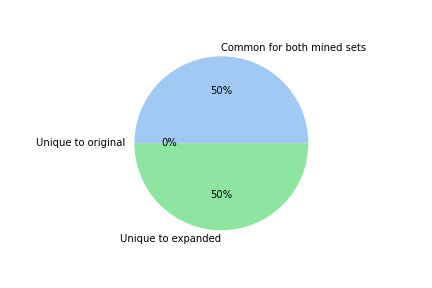
\includegraphics[width=\textwidth]{figures/results/entity_selection/pie_charts/probabilistic_wn18rr.png}
            \caption[complEx_pie]%
            {{\small Probabilistic}}    
            \label{fig:probabilistic_pie_wn18rr}
        \end{subfigure}
        \hfill
        \begin{subfigure}[b]{0.49\textwidth}  
            \centering 
            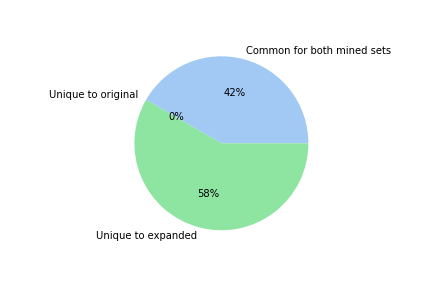
\includegraphics[width=\textwidth]{figures/results/entity_selection/pie_charts/random_wn18rr.png}
            \caption[]%
            {{\small Random}}    
            \label{random_pie_wn18rr}
        \end{subfigure}
        \vskip\baselineskip
        \begin{subfigure}[b]{0.49\textwidth}   
            \centering 
            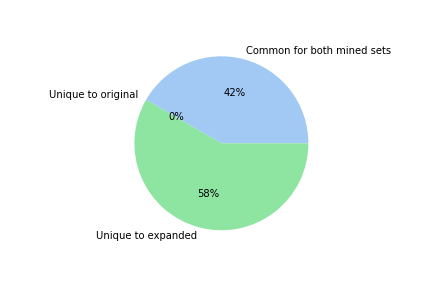
\includegraphics[width=\textwidth]{figures/results/entity_selection/pie_charts/most_frequent_wn18rr.png}
            \caption[]%
            {{\small Most Frequent}}    
            \label{fig:most_pie_wn18rr}
        \end{subfigure}
        \hfill
        \begin{subfigure}[b]{0.49\textwidth}   
            \centering 
            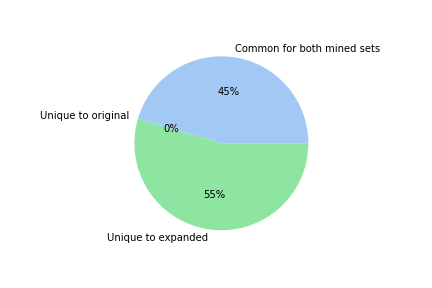
\includegraphics[width=\textwidth]{figures/results/entity_selection/pie_charts/least_frequent_wn18rr.png}
            \caption[]%
            {{\small Least Frequent}}    
            \label{fig:least_pie_wn18rr}
        \end{subfigure}
        \caption[]
        {\small Distribution of all the rules mined over entity selection strategies for WN18RR.} 
        \label{fig:entity_pies_wn18rr}
    \end{figure*}
    
    
    \begin{figure*}[h]
        \centering
        \begin{subfigure}[b]{0.49\textwidth}
            \centering
            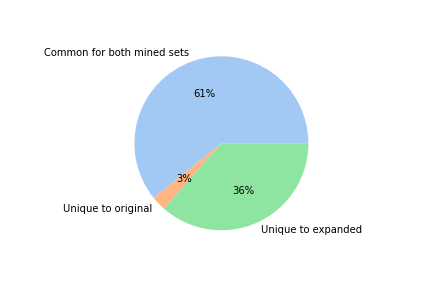
\includegraphics[width=\textwidth]{figures/results/entity_selection/pie_charts/Probabilistic_selection_family.png}
            \caption[]%
            {{\small Probabilistic}}    
            \label{fig:probablilistic_pie_family}
        \end{subfigure}
        \hfill
        \begin{subfigure}[b]{0.49\textwidth}  
            \centering 
            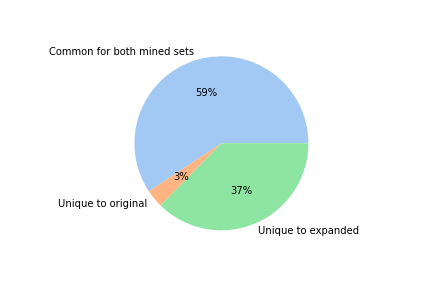
\includegraphics[width=\textwidth]{figures/results/entity_selection/pie_charts/random_family.png}
            \caption[]%
            {{\small Random}}    
            \label{fig:random_pie_family}
        \end{subfigure}
        \vskip\baselineskip
        \begin{subfigure}[b]{0.49\textwidth}   
            \centering 
            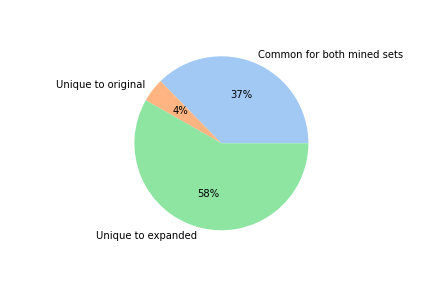
\includegraphics[width=\textwidth]{figures/results/entity_selection/pie_charts/most_frequent_family.png}
            \caption[]%
            {{\small Most Frequent}}    
            \label{fig:most_pie_family}
        \end{subfigure}
        \hfill
        \begin{subfigure}[b]{0.49\textwidth}   
            \centering 
            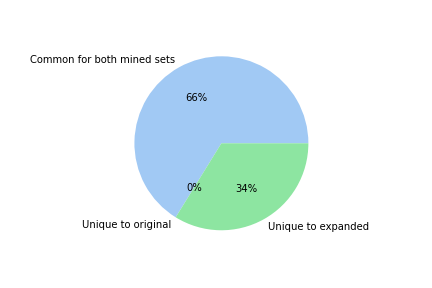
\includegraphics[width=\textwidth]{figures/results/entity_selection/pie_charts/least_frequent_family.png}
            \caption[]%
            {{\small Least Frequent}}    
            \label{fig:least_pie_family}
        \end{subfigure}
        \caption[]
        {\small Distribution of all the rules mined over entity selection strategies for the family KG.} 
        \label{fig:entity_pies_family}
    \end{figure*}

\fi




\newpage
\subsection{Effect of rank cutoff value}
Rank cutoff values determine which candidates are admitted to the KG. Only those with rank on the cutoff or above are accepted. Therefore, the lower the rank cutoff, the more candidates are added to the KG. The box plots in \cref{rank_extensions_boxplot} show evidence of this. The pie charts in figures \ref{rank_pies_family} and \ref{rank_pies_wn18rr} both show that when the rank cutoff was 1, all the original rules were found. Decrease in rank cutoff led to the mining of more new rules, but  also led to some original rules not being mined, especially in the WN18RR case. PCA confidence-wise the rank cutoff values had a slightly different effect on the two datasets. In the WN18RR dataset there was little difference in PCA confidence over the ranks when calculated over the original KG, while for the family KG the PCA confidence was increased at rank cutoff 4 and 7, with no change at rank cutoff 1. When calculated over the KG extensions rank 1 and 4 did worse than the mean of the original rules, while rank cutoff 7 did significantly better. On the family KG PCA confidence calculated on the extended KGs led to little variety over the rank values. Rank 1 resulted on the same median as the original rules, rank 4 just above and rank 7 just below. Overall it seems like if the goal is to find many new rules, then a higher rank cutoff values is more appropriate.

\begin{figure}[h]
\centering
\begin{subfigure}{.5\textwidth}
  \centering
  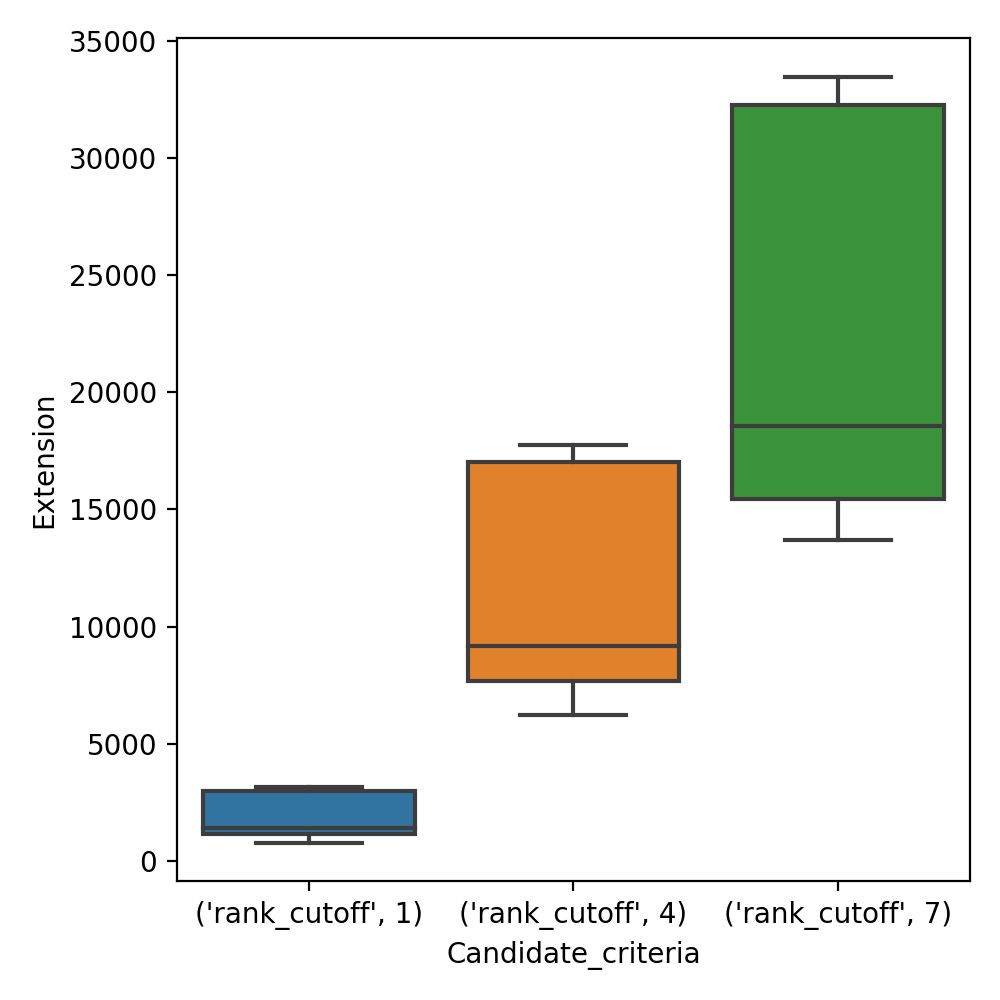
\includegraphics[width=1\linewidth]{figures/results/ranks/Extension_size_entity_wn18rr.png}
  \caption{WN18RR KG.}
  \label{fig:rank_extension_wn18rr_boxplot_sub}
\end{subfigure}%
\begin{subfigure}{.5\textwidth}
  \centering
  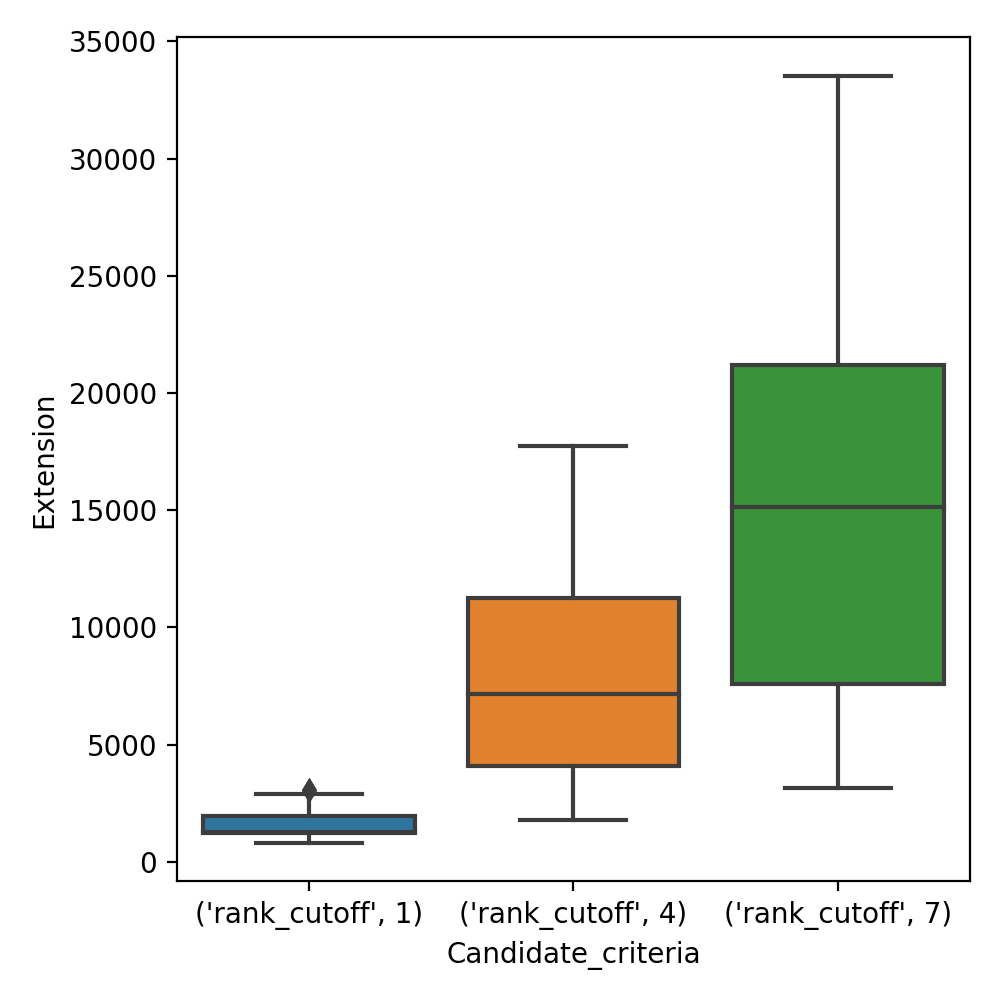
\includegraphics[width=1\linewidth]{figures/results/ranks/Extension_size_entity_family.png}
  \caption{Family KG.}
  \label{fig:rank_extension_family_boxplot_sub}
\end{subfigure}
\caption{Distribution of KG extension sizes over rank cutoff values.}
\label{rank_extensions_boxplot}
\end{figure}

\begin{figure}[h]
\centering
\begin{subfigure}{.5\textwidth}
  \centering
  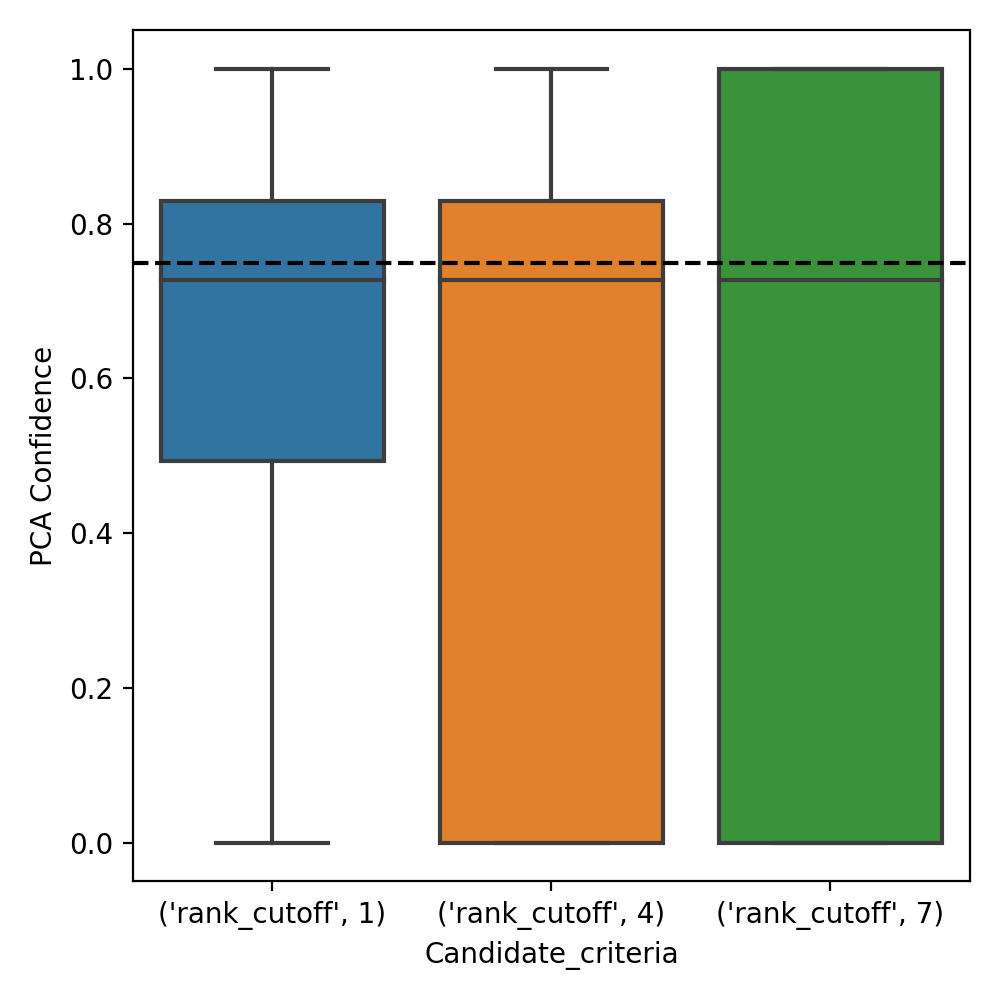
\includegraphics[width=1\linewidth]{figures/results/ranks/PCA-rank_wn18rr.png}
  \caption{Original KG}
  \label{fig:PCA-rank_wn18rr_boxplot_sub}
\end{subfigure}%
\begin{subfigure}{.5\textwidth}
  \centering
  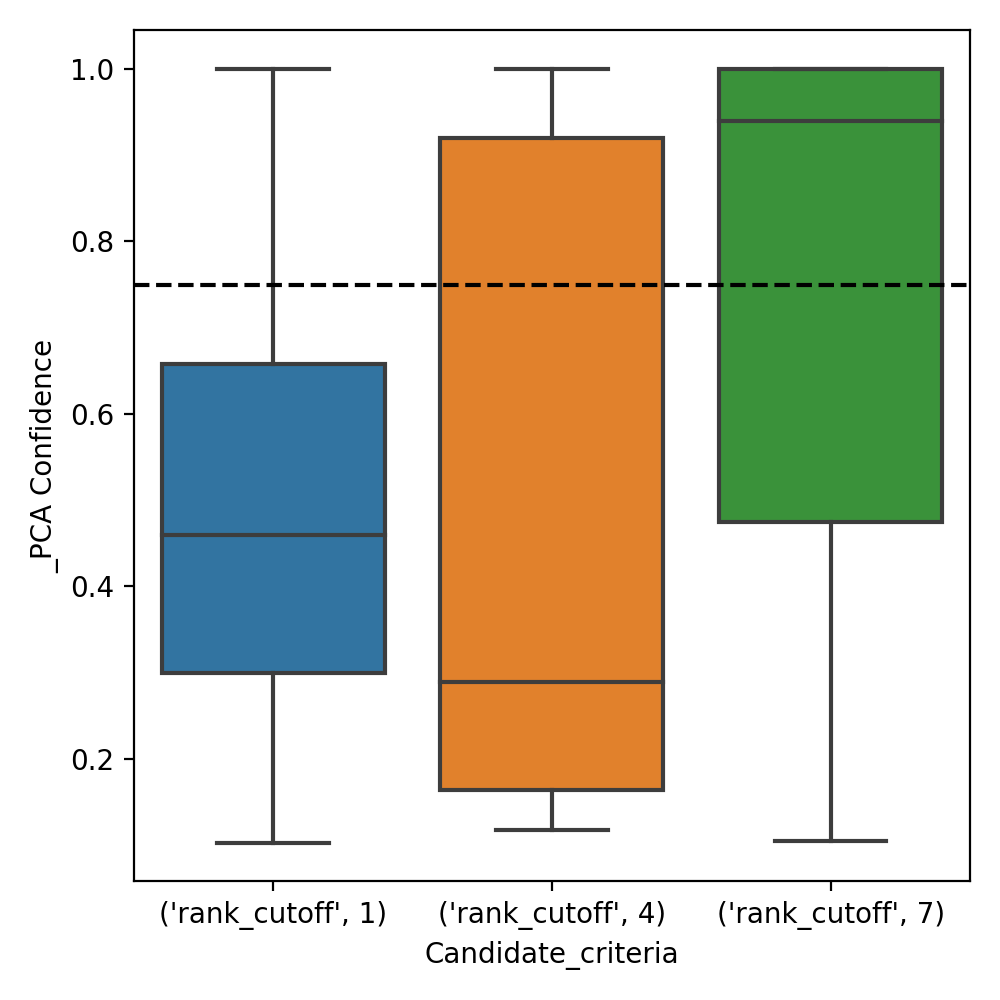
\includegraphics[width=1\linewidth]{figures/results/ranks/_PCA-rank_wn18rr.png}
  \caption{Extended KG}
  \label{fig:_PCA_rank_wn18rr_boxplot_sub}
\end{subfigure}
\caption{Distribution of PCA confidence of mined rules over rank cutoff values. PCA confidence scores are calculated on the original WN18RR and the extended WN18RR from which the rules are mined. The dashed line represents the median PCA confidence of the rules mined from the original WN18RR KG.}
\label{fig:PCA_rank_wn18rr_boxplot}
\end{figure}

\begin{figure}[h]
\centering
\begin{subfigure}{.5\textwidth}
  \centering
  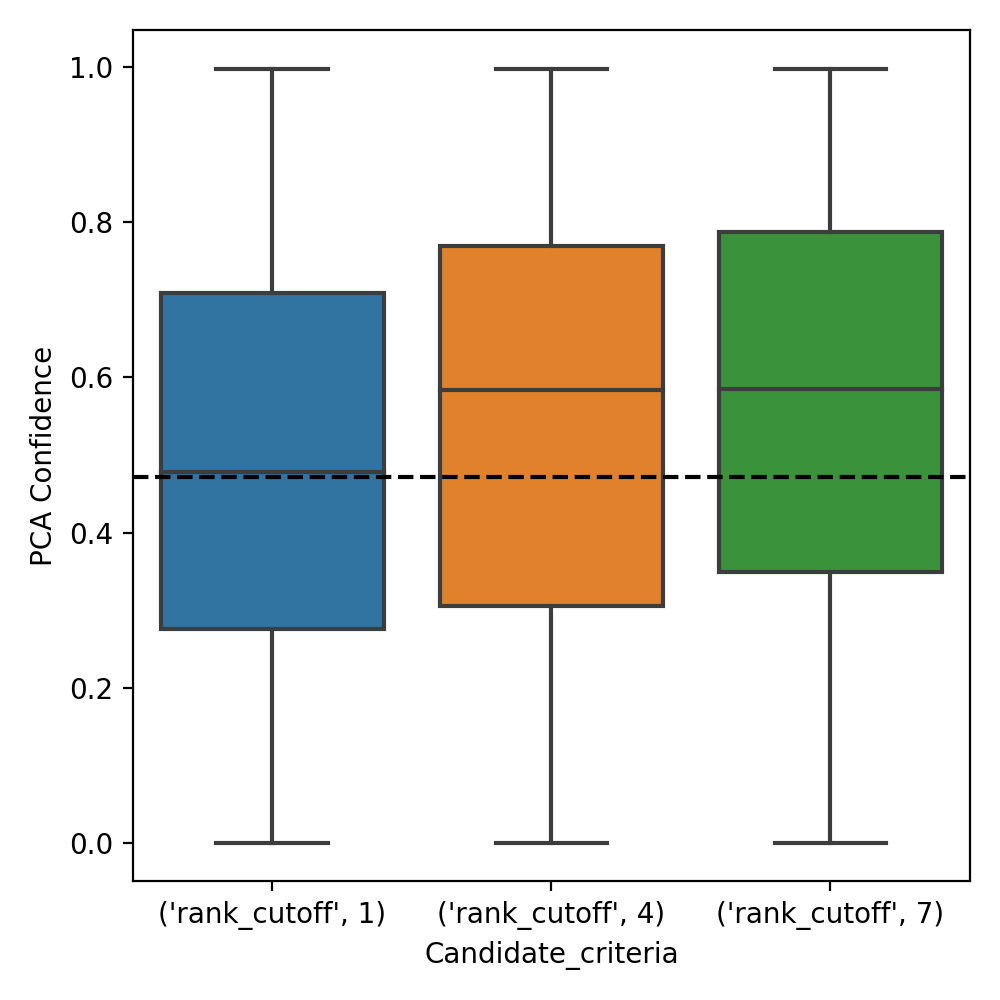
\includegraphics[width=1\linewidth]{figures/results/ranks/PCA-rank_family.png}
  \caption{Original KG}
  \label{fig:models_rank_boxplot_sub}
\end{subfigure}%
\begin{subfigure}{.5\textwidth}
  \centering
  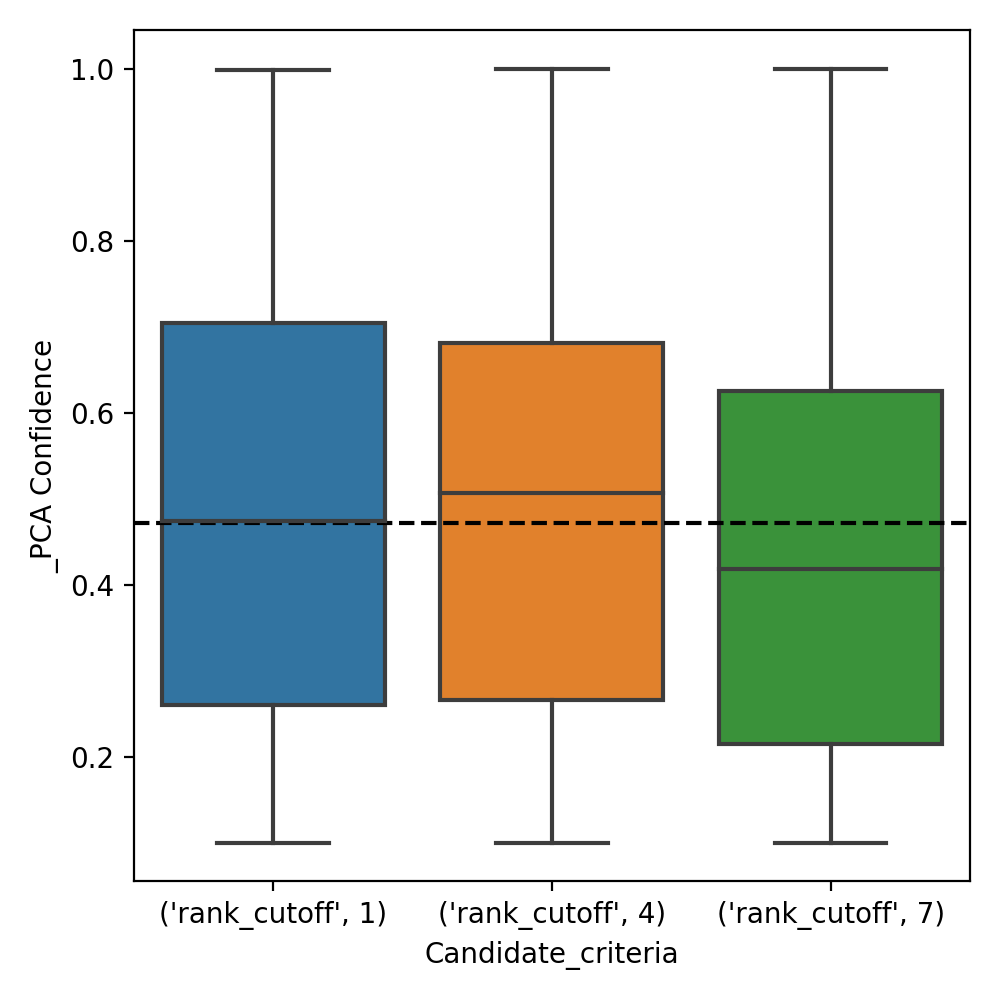
\includegraphics[width=1\linewidth]{figures/results/ranks/_PCA-rank_family.png}
  \caption{Extended KG}
  \label{fig:_PCA_rank_family_boxplot_sub}
\end{subfigure}
\caption{Distribution of PCA confidence of mined rules by rank cutoff values. PCA confidence scores are calculated on the original family KG and the extended family KG from which the rules are mined. The dashed line represents the median PCA confidence of the rules mined from the original family KG.}
\label{fig:PCA_entity_family_boxplot}
\end{figure}







\begin{figure*}[h]
        \centering
        \begin{subfigure}[b]{0.3\textwidth}
            \centering
            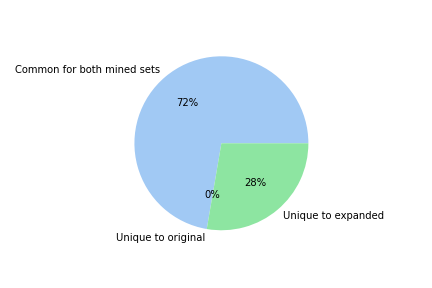
\includegraphics[width=\textwidth]{figures/results/ranks/pie_charts/('rank_cutoff', 1)_family.png}
            \caption[]%
            {{\small Rank 1}}    
            \label{fig:rank_1_pie_family}
        \end{subfigure}
        %\hfill
        \begin{subfigure}[b]{0.3\textwidth}  
            \centering 
            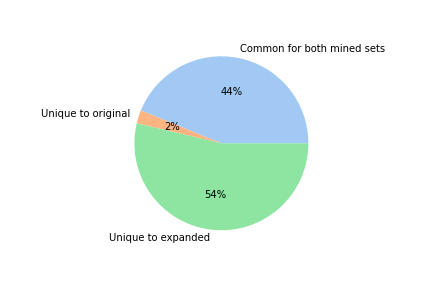
\includegraphics[width=\textwidth]{figures/results/ranks/pie_charts/('rank_cutoff', 4)_family.png}
            \caption[]%
            {{\small Rank 4}}    
            \label{fig:rank_4_pie_family}
        \end{subfigure}
        %\vskip\baselineskip
        \begin{subfigure}[b]{0.3\textwidth}   
            \centering 
            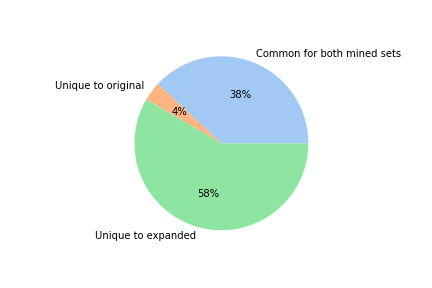
\includegraphics[width=\textwidth]{figures/results/ranks/pie_charts/('rank_cutoff', 7)_family.png}
            \caption[]%
            {{\small Rank 7}}    
            \label{fig:rank_1_pie_family}
        \end{subfigure}
        \hfill
        \caption[]
        {\small Distribution of all the rules mined over KG rank cutoff values. KG: family KG.} 
        \label{rank_pies_family}
    \end{figure*}
    
    
    \begin{figure*}[h]
        \centering
        \begin{subfigure}[b]{0.3\textwidth}
            \centering
            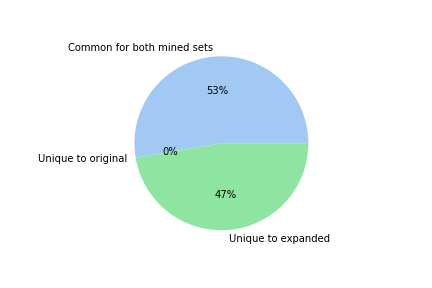
\includegraphics[width=\textwidth]{figures/results/ranks/pie_charts/('rank_cutoff', 1)_wn18rr.png}
            \caption[]%
            {{\small Rank 1}}    
            \label{fig:rank_1_pie_wn18rr}
        \end{subfigure}
        %\hfill
        \begin{subfigure}[b]{0.3\textwidth}  
            \centering 
            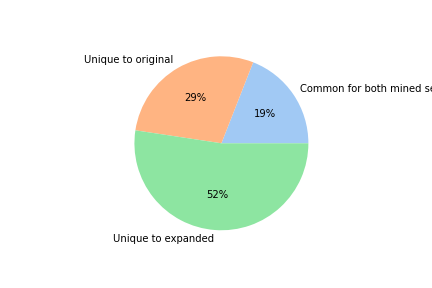
\includegraphics[width=\textwidth]{figures/results/ranks/pie_charts/('rank_cutoff', 4)_wn18rr.png}
            \caption[]%
            {{\small Rank 4}}    
            \label{fig:rank_4_pie_wn18rr}
        \end{subfigure}
       % \vskip\baselineskip
        \begin{subfigure}[b]{0.3\textwidth}   
            \centering 
            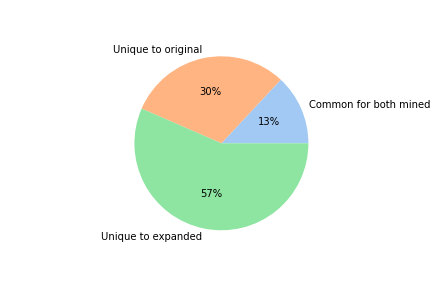
\includegraphics[width=\textwidth]{figures/results/ranks/pie_charts/('rank_cutoff', 7)_wn18rr.png}
            \caption[]%
            {{\small Rank 7}}    
            \label{fig:rank_7_pie_wn18rr}
        \end{subfigure}
        \hfill
        \caption[ ]
        {\small Distribution of all the rules mined over rank cutoff values. KG: WN18RR.} 
        \label{rank_pies_wn18rr}
    \end{figure*}
    

\newpage
\section{Rule comparison}
\label{Rule_comparison}
